From the technical reference:

ESP32-C6 is an ultra-low power and highly-integrated system that integrates:
\begin{itemize}
\item a high-performance 32-bit RISC-V single-core processor (HP CPU), four-stage pipeline, clock frequency
up to 160 MHz
\item a low-power 32-bit RISC-V single-core processor (LP CPU), two-stage pipeline, clock frequency up to
20 MHz
\end{itemize}
All internal memory, external memory, and peripherals are located on the HP CPU and LP CPU buses.

Features:
\begin{itemize}
\item Address Space
	\begin{itemize}
	\item 832 KB of internal memory address space accessed from the instruction bus or data bus
	\item 832 KB of peripheral address space
	\item 16 MB of external memory virtual address space accessed from the instruction bus or the data bus
	\item 512 KB of internal DMA address space
	\end{itemize}
\item Internal Memory
	\begin{itemize}
	\item 320 KB internal ROM
	\item 512 KB HP SRAM
	\item 16 KB LP SRAM
	\end{itemize}
\item External Memory
	\begin{itemize}
	\item Supports up to 16 MB external flash
	\end{itemize}
\item Peripheral Space
	\begin{itemize}
	\item 51 modules/peripherals in total
	\end{itemize}
\item GDMA
	\begin{itemize}
	\item 8 GDMA-supported modules/peripherals
	\end{itemize}
\end{itemize}

Here is a simplified diagram of the ESP32-C6's memory map.

\tikzset{every node/.append style={align=left, font=\LARGE}}
\tikzset{reserved/.style={fill=gray!30}}

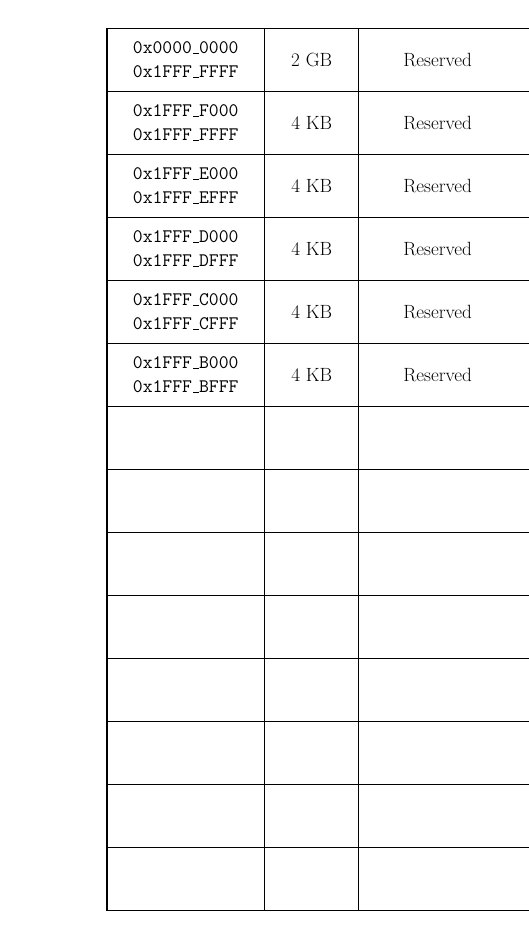
\begin{tikzpicture}[scale=0.4, every node/.append style={transform shape}]
\hspace*{1cm}
\draw (0,0) rectangle (15,-28);
% First column, address range
\draw (5,0) -- (5,-28);
% Second column, size 
\draw (8,0) -- (8,-28);
% Third column, title, from 8 to 15

% draw a row every 2 units from (0,i) to (15,i)
\foreach \i in {0,-2,...,-28}
	\draw (0,\i) -- (15,\i);

\node at (2.5,-1) {\texttt{0x0000\_0000}\\\texttt{0x1FFF\_FFFF}};
\node at (6.5,-1) {2 GB};
\node at (10.5,-1) {Reserved};

\node at (2.5,-3) {\texttt{0x1FFF\_F000}\\\texttt{0x1FFF\_FFFF}};
\node at (6.5,-3) {4 KB};
\node at (10.5,-3) {Reserved};

\node at (2.5,-5) {\texttt{0x1FFF\_E000}\\\texttt{0x1FFF\_EFFF}};
\node at (6.5,-5) {4 KB};
\node at (10.5,-5) {Reserved};

\node at (2.5,-7) {\texttt{0x1FFF\_D000}\\\texttt{0x1FFF\_DFFF}};
\node at (6.5,-7) {4 KB};
\node at (10.5,-7) {Reserved};

\node at (2.5,-9) {\texttt{0x1FFF\_C000}\\\texttt{0x1FFF\_CFFF}};
\node at (6.5,-9) {4 KB};
\node at (10.5,-9) {Reserved};

\node at (2.5,-11) {\texttt{0x1FFF\_B000}\\\texttt{0x1FFF\_BFFF}};
\node at (6.5,-11) {4 KB};
\node at (10.5,-11) {Reserved};

\end{tikzpicture}

And here follows another ...
